\documentclass[10pt,a4paper]{article}
\usepackage[utf8]{inputenc}
\usepackage{amsmath}
\usepackage{amsfonts}
\usepackage{amssymb}
\usepackage{graphicx}
\usepackage{multicol}
\usepackage[margin=1in]{geometry}

\title{Makespan Schedule Explanation Questionnaire}
\date{}
\author{}

\begin{document}
\maketitle
\vspace{-4\baselineskip}
\noindent\hrulefill

\noindent This questionnaire should take around five minutes. This will judge the general ability to understand and explain makespan schedule. Makespan schedules consist of $m$ machines and $n $ jobs. Every job is assigned to only one machine for the schedule to be feasible. Each job has a processing time. The objective is to minimise the longest collective processing time. Machines and jobs are denoted by integers $1,2,3,...$ and by letters $A,B,C,...$, respectively. A schedule is optimal when the longest collective processing time cannot be faster.

\begin{multicols}{2}
	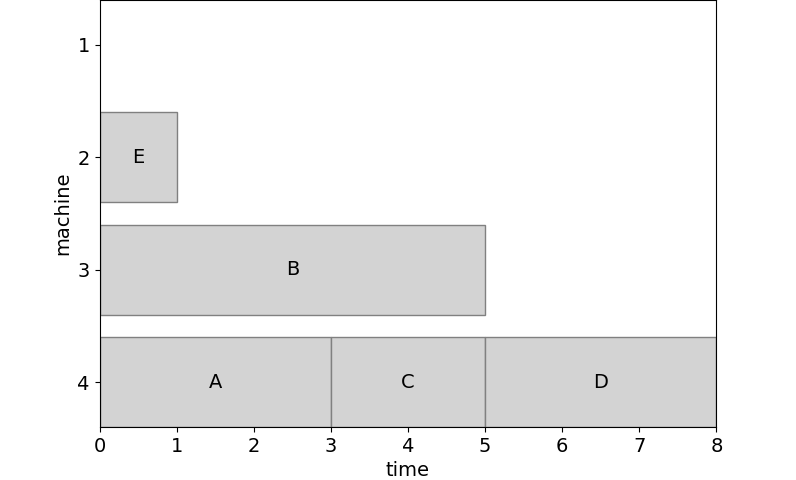
\includegraphics[width=0.5\textwidth]{figures/makespan_unoptimal}
	\begin{center}
		Schedule is not optimal because jobs $A,C,D$ can be moved to machine $1$.
	\end{center}
	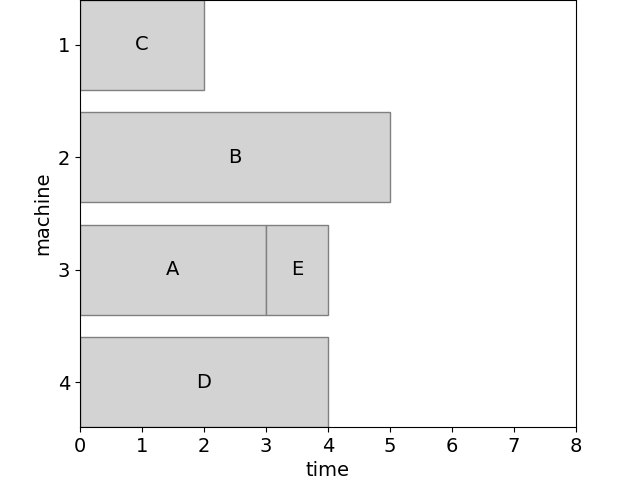
\includegraphics[width=0.4\textwidth]{figures/makespan_optimal}
	\begin{center}
		Schedule is optimal no assignment can be improved.
	\end{center}
\end{multicols}

\vspace{-\baselineskip}
\noindent\hrulefill

\noindent Aim to spend at most one minute for each question. Some questions are difficult. Write your answers in the boxes.

\begin{enumerate}
	\item This schedule is not optimal. Suggest steps required to optimise this schedule.

	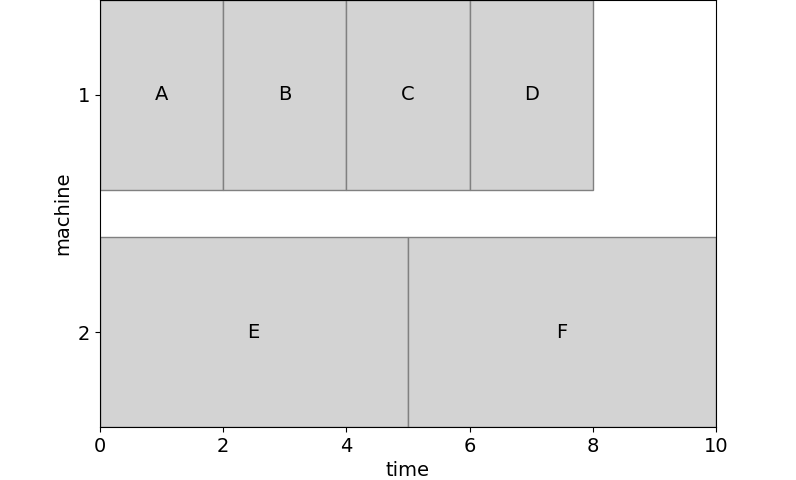
\includegraphics[width=0.5\textwidth]{figures/makespan_question1}\fbox{\rule{0.4\textwidth}{0pt}\rule{0pt}{4.7cm}}
	\item Is this schedule optimal? If not, suggest how it could be improved immediately.
	
	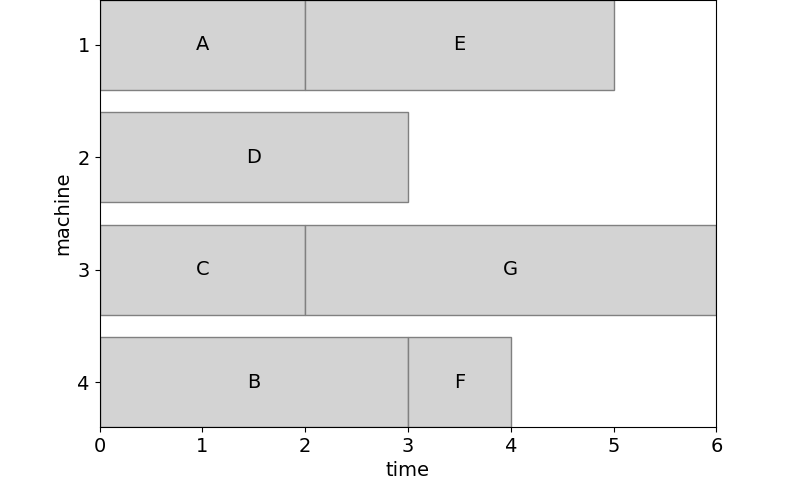
\includegraphics[width=0.5\textwidth]{figures/makespan_question2}\fbox{\rule{0.4\textwidth}{0pt}\rule{0pt}{4.7cm}}
	\item This schedule is optimal. Job $A$ cannot be assigned to machine $1$ or $2$ anymore. How could the schedule be modified to agree with this constraint?

	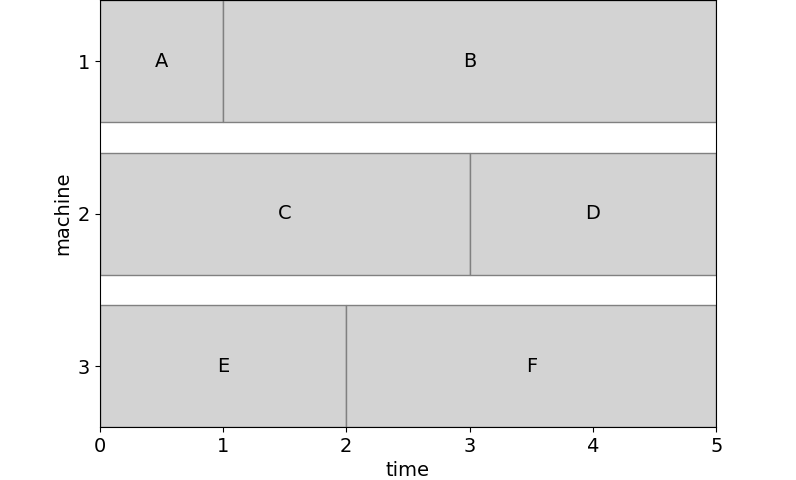
\includegraphics[width=0.5\textwidth]{figures/makespan_question3}\fbox{\rule{0.4\textwidth}{0pt}\rule{0pt}{4.7cm}}
	\item Either jobs $C$ and $D$, or jobs $B$ and $E$ must be assigned to the same machine. Which constraint is results in a better schedule, and why?

	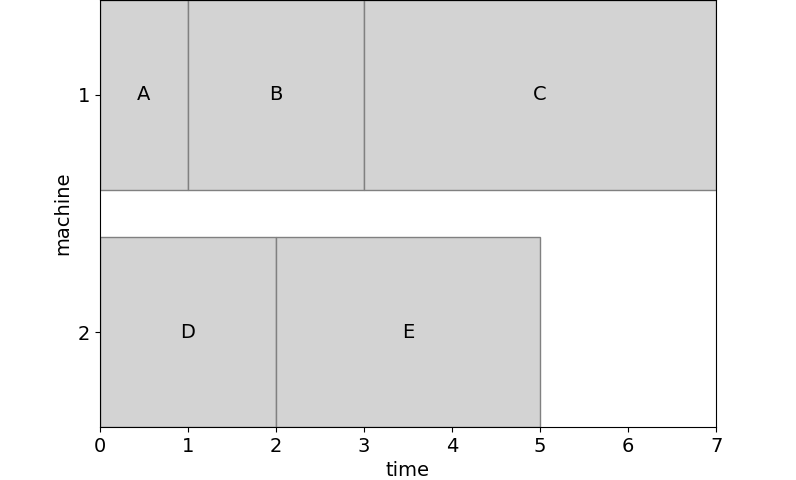
\includegraphics[width=0.5\textwidth]{figures/makespan_question4}\fbox{\rule{0.4\textwidth}{0pt}\rule{0pt}{4.7cm}}
	\item A new job $H$ of 5 time units needs to be scheduled. How could the schedule be modified to best accommodate this job?

	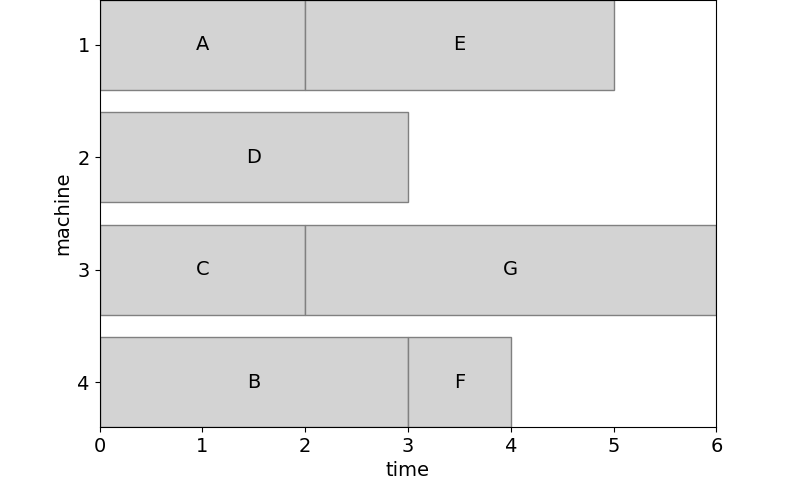
\includegraphics[width=0.5\textwidth]{figures/makespan_question2}\fbox{\rule{0.4\textwidth}{0pt}\rule{0pt}{4.7cm}}
\end{enumerate}

Thank you for your time. Please send your answers to \verb|myles.lee15@imperial.ac.uk|.

\end{document}
